\documentclass[a4paper]{article}
\usepackage{graphicx} % Required to insert images
\usepackage{amsmath}  % align, \text, \eqref
\usepackage{float}    % [H]: figure e tabelle restano dove le metto nel testo
\usepackage{url}
\usepackage{siunitx}
\renewcommand{\tablename}{Tabella}
\renewcommand{\figurename}{Figura}
\renewcommand{\refname}{Bibliografia}

\title{Pendolo Fisico}
\author{Cristiano Battini (729924)\quad
        \vspace{3mm}
        Francesco Micera (735172)\\
        gruppo A2-3\quad tavolo 2}
\date{Data dell'esperienza: 3 Novembre 2026\\
      Data di completamento relazione: 8 Novembre 2026}

\begin{document}

\maketitle
\section{Scopo dell'Esperienza}\label{sec:scopo}
In questa esperienza abbiamo verificato come il periodo di oscillazione di un pendolo fisico dipende dalla distanza d tra l’asse di rotazione e il centro di massa. Un pendolo fisico è un qualsiasi corpo rigido libero di oscillare, sotto l’azione della forza di gravità, attorno a un asse orizzontale fisso che non passa per il suo centro di massa. Nel nostro caso il corpo rigido è un’asta metallica forata e l’asse di rotazione è il perno su cui viene appesa. Per verificare questa dipendenza abbiamo misurato il periodo di oscillazione sospendendo l’asta ai diversi fori, quindi a diverse distanze dal centro di massa. Abbiamo poi confrontato i dati con il modello teorico~\eqref{eq:periodo}. I dati sono stati inseriti nel modello lasciando la lunghezza l come unico parametro libero. Il valore di best-fit è stato poi confrontato con la lunghezza dell’asta misurata direttamente. L’accordo del modello con i dati è stato inoltre valutato tramite l’analisi dei residui.


\section{Cenni Teorici}\label{sec:cenni_teorici}
Si definisce pendolo fisico un corpo rigido vincolato a ruotare, sotto l’azione della gravità, attorno a un asse orizzontale fisso che non passa per il suo centro di massa. Sia P il punto di sospensione, d la distanza tra P e il centro di massa, e $\theta$ l’angolo che il segmento che li congiunge forma con la verticale. Rispetto a P, il momento della forza peso agisce come se tutta la massa si trovasse nel centro di massa, quindi $\vec\tau = \vec r_{\mathrm{cm}} \times m\vec g$, dove la sua componente lungo l’asse di rotazione vale
\begin{equation}
    \tau = -mgd\,\sin\theta .
    \label{eq:momento_peso}
\end{equation}
Il segno negativo esprime il carattere di richiamo del momento, che tende sempre a riportare il sistema nella posizione di equilibrio stabile $\theta$ = 0.
Per un corpo rigido in rotazione attorno a un asse fisso, il momento angolare rispetto all’asse è $L = I\omega = I\,\dot\theta$, dove I è il momento d’inerzia rispetto all’asse passante per P. La seconda equazione cardinale della dinamica dà allora
\begin{equation}
    \tau = \frac{dL}{dt} = I\,\frac{d^2\theta}{dt^2},
    \label{eq:seconda_cardinale}
\end{equation}
e quindi, combinando la~\eqref{eq:seconda_cardinale} con la~\eqref{eq:momento_peso},
\begin{equation}
    \frac{d^2\theta}{dt^2} + \frac{mgd}{I}\,\sin\theta = 0.
    \label{eq:moto}
\end{equation}
Questa equazione non è lineare e non ammette soluzione in termini di funzioni elementari. Si ricorre quindi all’approssimazione di piccole oscillazioni. Dallo sviluppo in serie di Taylor $\sin\theta = \theta - \theta^3/6 + O(\theta^5)$, la sostituzione $\sin\theta \simeq \theta$ comporta un errore relativo dell’ordine di $\theta^2/6$. L’approssimazione è quindi lecita per $|\theta| \ll 1$ rad: per esempio, a 10° l’errore è circa lo $0.5\%$. Sostituendo nella~\eqref{eq:moto} si ottiene così:
\begin{equation}
    \frac{d^2\theta}{dt^2} + \frac{mgd}{I}\,\theta = 0,
    \label{eq:moto_lineare}
\end{equation}
cioè l’equazione di un oscillatore armonico, con pulsazione e periodo
\begin{equation}
    \omega_0 = \sqrt{\frac{mgd}{I}}, \qquad T_0 = \frac{2\pi}{\omega_0} = 2\pi\sqrt{\frac{I}{mgd}}.
    \label{eq:omega_T0}
\end{equation}
Il pendolo semplice si ritrova come caso particolare, con la massa concentrata a distanza d dal polo: $I = md^2$, quindi $T_0 = 2\pi\sqrt{d/g}$. In questo caso il periodo non dipende né dalla massa né dall’ampiezza (isocronismo delle piccole oscillazioni).

Per l’asta il momento d’inerzia si calcola con il teorema di Huygens-Steiner, che lo lega a quello rispetto all’asse parallelo passante per il centro di massa:
\begin{equation}
    I = I_{\mathrm{cm}} + md^2 = \frac{ml^2}{12} + md^2,
    \label{eq:steiner}
\end{equation}
dove l’ultima uguaglianza vale per un’asta sottile e omogenea di lunghezza l. Sostituendo la~\eqref{eq:steiner} nell’espressione di $T_0$ della~\eqref{eq:omega_T0}, la massa si semplifica e si ottiene il modello da verificare:
\begin{equation}
    T(d) = 2\pi\sqrt{\frac{l^2/12 + d^2}{g\,d}} .
    \label{eq:periodo}
\end{equation}
Questo modello vale solo dentro le ipotesi introdotte. Se l’ampiezza $\theta_0$ non è trascurabile, il periodo della soluzione della~\eqref{eq:moto} ammette il seguente sviluppo di Taylor:
\begin{equation}
    T(\theta_0) = T_0\left(1 + \frac{\theta_0^2}{16} +  \dots\right).
    \label{eq:sviluppo_ampiezza}
\end{equation}
Il termine dominante è $\theta_0^2/16$, e questo ci risulterà utile per delle considerazioni sui materiali usati nell'esperienza (sezione~\ref{sec:misure_dirette}).
\subsection{Incertezze di misura}

Ogni misura che facciamo ha un'incertezza, che ci dice entro quale intervallo ci aspettiamo che stia il valore vero. Nel nostro caso le incertezze vengono soprattutto da due cose: la risoluzione degli strumenti, che non ci permette di leggere valori pi\`u piccoli di una certa soglia, e le piccole differenze tra una misura e l'altra, dovute in gran parte al tempo di reazione quando facciamo partire e fermiamo il cronometro a mano. Qui spieghiamo come abbiamo stimato le incertezze sulle misure dirette e come le abbiamo poi portate fino alle grandezze calcolate e al risultato del fit. Gli eventuali errori sistematici non sono inclusi in queste incertezze, e ne parliamo nelle conclusioni.

Quando una grandezza l'abbiamo misurata una volta sola, o quando ripetendo la misura ottenevamo sempre lo stesso valore, abbiamo usato come incertezza la risoluzione dello strumento: 1~mm per il metro a nastro, 0.05~mm per il calibro ventesimale e 0.01~s per il cronometro.

Per i tempi invece le misure cambiavano un po' ogni volta, quindi le abbiamo ripetute pi\`u volte. Come valore abbiamo preso la media delle $n$ misure,
\begin{equation}
    \bar{x} = \frac{1}{n}\sum_{k=1}^{n} x_k ,
\end{equation}
e come incertezza la deviazione standard della media,
\begin{equation}
    \sigma_{\bar{x}} = \sqrt{\frac{1}{n(n-1)}\sum_{k=1}^{n} (x_k - \bar{x})^2} ,
\end{equation}
che tiene conto di quanto le misure sono sparpagliate attorno alla media e di quante ne abbiamo fatte.

Alcune grandezze non le abbiamo misurate direttamente, ma le abbiamo calcolate a partire da altre misure, quindi la loro incertezza va ricavata da quella delle misure di partenza. Nella nostra esperienza ci sono serviti solo due casi. Se una grandezza \`e la somma o la differenza di misure indipendenti, $G = x \pm y \pm z$, le incertezze si sommano in quadratura:
\begin{equation}
    \sigma_G = \sqrt{\sigma_x^2 + \sigma_y^2 + \sigma_z^2} .
\end{equation}
\`E il caso della distanza $d$, che otteniamo come differenza di tre lunghezze. Se invece una grandezza \`e una misura moltiplicata per un numero esatto, $G = c\,x$, anche l'incertezza va moltiplicata per lo stesso numero:
\begin{equation}
    \sigma_G = |c|\,\sigma_x .
\end{equation}
Questo l'abbiamo usato per il periodo, che otteniamo dividendo per 10 il tempo di dieci oscillazioni, e per la posizione del centro di massa e il raggio del foro, che sono la met\`a della lunghezza dell'asta e del diametro del foro. Sempre in quadratura abbiamo poi sommato l'incertezza statistica sul periodo e l'errore di lettura del cronometro, visto che sono indipendenti tra loro.

L'incertezza sulla lunghezza ottenuta dal fit la prendiamo dalla matrice di covarianza che restituisce il programma: \`e la radice dell'elemento sulla diagonale. Siccome nel fit abbiamo usato le nostre incertezze sperimentali cos\`i come sono, senza riscalarle, questa incertezza dipende solo da quelle che abbiamo assegnato ai periodi.

Infine, per capire se due misure della stessa grandezza vanno d'accordo, come la lunghezza dal fit e quella misurata con il metro, calcoliamo
\begin{equation}
    z = \frac{|a - b|}{\sqrt{\sigma_a^2 + \sigma_b^2}} ,
\end{equation}
che ci dice di quante deviazioni standard differiscono le due misure.

\section{Materiali e Strumenti di Misura}\label{sec:materiali}
%\section{Apparato Strumentale} %da utilizzare quando l'apparato è più complesso
L'esperienza consiste nel misurare i tempi di oscillazione del pendolo fisico e i materiali e gli strumenti di misurazione usati sono stati:
\begin{itemize}
    \item un'asta metallica forata,
    \item un supporto di sospensione
    \item un calibro ventesimale, risoluzione 0.05 mm
    \item metro a nastro, risoluzione 1 mm
    \item cronometro, risoluzione 0.01 s
\end{itemize}

\section{Misure Dirette}\label{sec:misure_dirette}
 Prima di iniziare a prendere le misure abbiamo analizzato l'asta metallica per verificare la posizione del centro di massa dell'asta considerando anche la presenza dei fori. Per fare questo abbiamo misurato per prima cosa le dimensioni dell'asta, profondità, larghezza con il calibro ventesimale e lunghezza con il metro a nastro. Infine abbiamo misurato il diametro dei fori.
 Dopo abbiamo verificato quanto effettivamente "pesassero" questi fori sulla posizione del centro di massa.
 Le misure sono riportate in tabella~\ref{tab:asta}.

\begin{table}[H]
    \centering
    \begin{tabular}{c|c|c}
      & misura (mm) & strumento\\
      \hline
      larghezza $b$ & $16.05 \pm 0.05$ & calibro \\
      profondità $p$ & $15.25 \pm 0.05$ & calibro \\
      lunghezza $l$ & $1051 \pm 1$ & metro \\
      diametro foro $2r$ & $4.90 \pm 0.05$ & calibro \\
    \end{tabular}
    \caption{Dimensioni dell'asta e dei fori. Come incertezza abbiamo preso la risoluzione dello strumento.}
    \label{tab:asta}
\end{table}

 Considerando che fori e asta hanno la stessa altezza e i solidi in questione come regolari possiamo procedere con i calcoli considerando solo l'area delle facce per trarre le nostre considerazioni.
 Con i valori della tabella~\ref{tab:asta}, l'area della faccia dell'asta e quella di un foro sono
\begin{equation}
    A_{asta} = b \cdot l = 16.05 \cdot 1051\ \text{mm}^2 \simeq 16869\ \text{mm}^2
    \label{eq:area_asta}
\end{equation}
\begin{equation}
    A_{foro} = \pi r^2 = \pi \cdot (2.45)^2\ \text{mm}^2 \simeq 18.86\ \text{mm}^2
    \label{eq:area_foro}
\end{equation}
e con n = 10 fori l'area totale dei fori è
\begin{equation}
    A_{fori} = n \cdot A_{foro} \simeq 188.6\ \text{mm}^2
    \label{eq:area_fori}
\end{equation}
Dalle~\eqref{eq:area_asta} e~\eqref{eq:area_fori} il rapporto è quindi
\begin{equation}
    \frac{A_{fori}}{A_{asta}} = \frac{188.6}{16869} \simeq 0.0112
    \label{eq:rapporto_aree}
\end{equation}
 Trovato che l'area dei fori, dove non abbiamo considerato l'altezza in quanto fori e asta hanno la stessa troviamo che l'area dei fori è circa 1\% dell'area totale dell'asta. \newline Abbiamo poi verificato come questa considerazione ricadesse sulla massa, poichè fori presenti sull’asta riducono la massa di quest'ultima, ma più notevolmente ne alterano la distribuzione, dunque il centro di massa.
 Il loro effetto sul periodo è però trascurabile. Trattando i fori come cilindri di raggio r, la frazione di massa rimossa rispetto all’asta piena è il rapporto della~\eqref{eq:epsilon}, lo indichiamo con la lettere epsilon:
\begin{equation}
    \varepsilon = 0.0112
    \label{eq:epsilon}
\end{equation}
La posizione dei vari fori può influire sul modello nello spostare il centro di massa.

I fori sono equidistanziati, con un passo di circa 100 mm, ma non sono disposti simmetricamente rispetto al centro dell’asta. Il centro del primo foro dista circa 43.3 mm dall’estremità superiore, mentre l’ultimo dista circa 100 mm dall’estremità inferiore. Di conseguenza il baricentro dei fori non coincide con il centro geometrico, ma è spostato verso l’estremità superiore di:
\begin{equation}
    s = \frac{1}{n}\sum_{k=1}^{n} x_k \simeq 26\ \text{mm},
    \label{eq:baricentro_fori}
\end{equation}
dove $x_k$ è la distanza del centro del k-esimo foro rispetto al centro geometrico dell’asta. La massa mancante è quindi sbilanciata verso l’alto, e combinando la~\eqref{eq:epsilon} con la~\eqref{eq:baricentro_fori} il centro di massa dell’asta forata si sposta verso il basso. 
\newline
Dato che la massa dell'asta piena sarebbe: asta piena = asta forata + materiale dei fori.
$$M \cdot x_{cm, piena} = (1-\varepsilon)M\, x_{cm, effettivo} + \varepsilon M\, s$$
Dove $x_{cm,piena}=0$ per definizione, e chiamiamo $x_{cm,effettivo}=\delta$, poichè rappresenta lo "shift" del centro di massa da quello se la massa dell'asta fosse stata omogenea coincidente con il centro geometrico. Inoltre possiamo eliminare tutti i termini $M$ della massa, poichè costanti, diversi da zero ed eliminabili da entrambi le parti.
$$0 = (1-\varepsilon)\delta + \varepsilon s$$
Da cui si ricava $\delta$:
\begin{equation}
    \delta = \frac{\varepsilon\, s}{1-\varepsilon} \simeq 0.3\ \text{mm}
    \label{eq:spostamento_cm}
\end{equation}
 Essendo questo inferiore a meno della metà dell'incertezza sulla lunghezza dell'asta che ricordiamo essere di 1 mm possiamo affermare che i fori siano trascurabili nella posizione del centro di massa.
Verificato quindi di poter calcolare il centro di massa geometricamente, questo risulta essere a metà di ogni dimensione dell'asta:
\begin{equation}
    C_m = (x, y, z) = \left(\frac{b}{2}, \frac{l}{2}, \frac{p}{2}\right) = (8.02 \pm 0.02,\ 525.5 \pm 0.5,\ 7.63 \pm 0.03)\ \text{mm}
    \label{eq:centro_massa}
\end{equation}
dove le incertezze si ottengono dividendo per 2 quelle degli strumenti, e abbiamo approssimato le incertezze con 0.025 una a 0.03 e una a 0.02, dunque alternatamente per ridurre le fluttuazioni statistiche.
In seguito abbiamo cercato le condizioni dove si potesse verificare l'ipotesi delle piccole oscillazioni nel nostro esperimento per darci un range nel quale far partire l'asta.
Tenendo a mente la~\eqref{eq:sviluppo_ampiezza}.
L’approssimazione è accettabile se il termine dominante è trascurabile rispetto all’incertezza con cui misuriamo il periodo, cioè se
\begin{equation}
    T_0\,\frac{\theta_0^2}{16} < \sigma_T \quad\Longrightarrow\quad \theta_0 < 4\sqrt{\frac{\sigma_T}{T_0}} .
    \label{eq:limite_ampiezza}
\end{equation}
Il limite dipende quindi dalla precisione relativa $\sigma_T$ /T raggiunta a ciascuna distanza.

Durante l'esperienza però abbiamo sbagliato questo calcolo: abbiamo confrontato il termine $\theta_0^2/16$, trascurando la grandezza $T_0$, \newline e ci veniva $\theta_0 < 0.4$ rad, cioè circa 23°. Rifacendo il conto nel modo giusto con la~\eqref{eq:limite_ampiezza} e con le nostre misure (tabella~\ref{tab:periodi}), per le quali $\sigma_T$ va da circa 1.6 ms a 4.4 ms, si ottiene un’ampiezza massima compresa tra $\theta_0 \approx $ 0.11 rad (6°) per $d_5$ e $\theta_0 \approx$ 0.21 rad (12°) per $d_1$.

Per controllare l’ampiezza iniziale, all’istante del rilascio abbiamo misurato con il metro lo spostamento orizzontale a di un punto dell’asta e la sua distanza h dal perno. L’angolo si ricava da
\begin{equation}
    \theta_0 = \arcsin\frac{a}{h}.
    \label{eq:angolo_iniziale}
\end{equation}
Per esempio, con a = 15 cm e h = 54 cm la~\eqref{eq:angolo_iniziale} dà $\theta_0 \approx$ 0.28 rad, cioè 16°. Durante le 10 oscillazioni cronometrate l’ampiezza diminuisce per effetto dell’attrito, quindi l’ampiezza media effettiva è un po’ minore di quella iniziale.
Quindi l'ampiezza con cui abbiamo fatto partire l'asta è più grande del limite che abbiamo trovato per tutte le distanze, e non possiamo considerare trascurabile l'effetto dell'ampiezza, poichè superiore alle piccole oscillazioni. Non potendo rifare le misure, lo abbiamo trattato come un errore sistematico nell'analisi dati (sezione~\ref{sec:ampiezza}).

Fatta questa premessa abbiamo cronometrato i tempi delle oscillazioni con diverse distanze, prendendo per ogni misura il periodo di 10 oscillazioni per abbattere sia l'errore dello strumento che l'errore umano nel prendere i tempi, che nel caso fossero stati presi a singola oscillazione avrebbero avuto un errore umano molto più grande. In seguito abbiamo misurato anche le distanze del centro di massa fissando i vari punti P al centro del foro, quindi sottraendo un raggio dal risultato.
Quindi per ogni foro la distanza dal centro di massa è
\begin{equation}
    d = \frac{l}{2} - x - r ,
    \label{eq:distanza}
\end{equation}
dove x è la distanza tra l'estremità superiore dell'asta e il bordo del foro. Le distanze $d_1$ e $d_2$ le abbiamo misurate con il calibro, mentre $d_3$, $d_4$ e $d_5$ con il metro. L'incertezza su d l'abbiamo ottenuta sommando in quadratura l'incertezza sul centro di massa (0.5 mm, equazione~\eqref{eq:centro_massa}) con quelle sulla misura di x e sul raggio del foro, e viene 0.5 mm per le misure con il calibro e 1.2 mm per quelle con il metro. Le misure dei tempi sono riportate in tabella~\ref{tab:misure}.

\begin{table}[H]
    \centering
    \small
    \begin{tabular}{c|c|c|c|c|c}
      & $d_1$ & $d_2$ & $d_3$ & $d_4$ & $d_5$ \\
      $d$ (mm) & $482.3 \pm 0.5$ & $375.2 \pm 0.5$ & $276.1 \pm 1.2$ & $176.0 \pm 1.2$ & $75.1 \pm 1.2$ \\
      \hline
      Tempo 1 (s) & 16.23 & 15.70 & 15.77 & 16.83 & 22.93 \\
      Tempo 2 (s) & 16.41 & 15.83 & 15.72 & 16.80 & 22.95 \\
      Tempo 3 (s) & 16.51 & 15.74 & 15.65 & 16.83 & 22.90 \\
      Tempo 4 (s) & 16.30 & 15.84 & 15.73 & 16.77 & 22.97 \\
      Tempo 5 (s) & 16.47 & 15.80 & 15.74 & 16.90 & 22.92 \\
      Tempo 6 (s) & 16.39 & - & - & - & - \\
    \end{tabular}
    \caption{Per ogni distanza dal centro di massa, varie misurazioni del tempo di N = 10 oscillazioni (in secondi). Incertezza sul tempo dello strumento coincidente con la risoluzione del cronometro 0.01 s.}
    \label{tab:misure}
\end{table}

\newpage

\section{Analisi dati}\label{sec:analisi}


\subsection{Metodologia}\label{sec:metodologia}
Per l'analisi dei dati abbiamo scritto un programma in Python, utilizzando
le librerie NumPy, SciPy e Matplotlib. Per ciascuna distanza $d_i$ abbiamo
diviso per $N = 10$ i tempi misurati (tabella~\ref{tab:misure}), ottenendo il periodo di ogni
ripetizione. Come valore centrale $T_i$ abbiamo preso la media delle
ripetizioni. Come incertezza $\sigma_{T_i}$ abbiamo preso la deviazione
standard della media, sommata in quadratura con l'errore di lettura del
cronometro sul singolo periodo
($0.01\,\mathrm{s}/10 = 0.001\,\mathrm{s}$).

Il fit dei punti $(d_i, T_i)$ con il modello~\eqref{eq:periodo}, avente $l$
come unico parametro libero, è stato eseguito con la funzione
\texttt{curve\_fit} di SciPy. Questa implementa il metodo dei minimi
quadrati non lineari, pesando ogni punto con l'inverso del quadrato
dell'incertezza, $w_i = 1/\sigma_{T_i}^2$. Le incertezze su $d_i$ non sono incluse nel fit e compaiono
solo come barre d'errore nei grafici.

Infine abbiamo confrontato il valore di best-fit $\hat{l}$ con la
lunghezza $l$ misurata direttamente, valutando la compatibilità tramite il
rapporto
\begin{equation}
  z = \frac{|\hat{l} - l|}{\sqrt{\sigma_{\hat{l}}^2 + \sigma_l^2}} ,
  \label{eq:z}
\end{equation}
e abbiamo analizzato i residui
\begin{equation}
  r_i = T_i - T(d_i;\hat{l})
  \label{eq:residui}
\end{equation}
in funzione di $d_i$.

\subsection{Risultati}\label{sec:risultati}

Per ogni distanza $d$ abbiamo calcolato il periodo di ogni ripetizione dividendo per 10 il tempo misurato, e poi la media e la sua incertezza come descritto nella sezione~\ref{sec:metodologia}. I risultati sono riportati in tabella~\ref{tab:periodi}.

\begin{table}[H]
    \centering
    \begin{tabular}{c|c|c|c}
      & $d\pm\sigma_d$ (mm) & n. ripetizioni & $T\pm\sigma_T$ (s)\\
      \hline
      $d_1$ & $482.3 \pm 0.5$ & 6 & $1.6385 \pm 0.0044$ \\
      $d_2$ & $375.2 \pm 0.5$ & 5 & $1.5782 \pm 0.0029$ \\
      $d_3$ & $276.1 \pm 1.2$ & 5 & $1.5722 \pm 0.0022$ \\
      $d_4$ & $176.0 \pm 1.2$ & 5 & $1.6826 \pm 0.0024$ \\
      $d_5$ & $75.1 \pm 1.2$  & 5 & $2.2934 \pm 0.0016$ \\
    \end{tabular}
    \caption{Valore centrale del periodo di oscillazione per ciascuna distanza $d$ tra il perno e il centro di massa. L'incertezza su $T$ è la deviazione standard della media, sommata in quadratura con l'errore di lettura del cronometro sul singolo periodo.}
    \label{tab:periodi}
\end{table}

\newpage
L'incertezza relativa sul periodo $\sigma_T/T$ va da circa $0.07\%$ per $d_5$ a circa $0.3\%$ per $d_1$.

\begin{table}[H]
    \centering
    \begin{tabular}{c|c|c}
      & $\sigma_T / T$ & in \% \\
      \hline
      $d_1$ & $2.7 \cdot 10^{-3}$ & 0.27\% \\
      $d_2$ & $1.8 \cdot 10^{-3}$ & 0.18\% \\
      $d_3$ & $1.4 \cdot 10^{-3}$ & 0.14\% \\
      $d_4$ & $1.4 \cdot 10^{-3}$ & 0.14\% \\
      $d_5$ & $7.0 \cdot 10^{-4}$ & 0.07\% \\
    \end{tabular}
    \caption{Incertezza relativa sul periodo di oscillazione per ciascuna distanza $d$, calcolata a partire dai valori di Tabella~\ref{tab:periodi}.}
    \label{tab:incertezze_relative}
\end{table}

La dispersione delle misure ripetute invece non è uguale per tutte le distanze: sul singolo periodo va da circa 3 ms per $d_5$ fino a circa 10 ms per $d_1$, che è la serie di misure più dispersa. In figura~\ref{fig:dispersione} riportiamo lo scarto di ogni misura dalla media del proprio gruppo: anche per $d_1$ nessuna misura si allontana dalla media più di circa una volta e mezza la deviazione standard, quindi non ci sono valori anomali da scartare.

\begin{figure}[H]
    \centering
    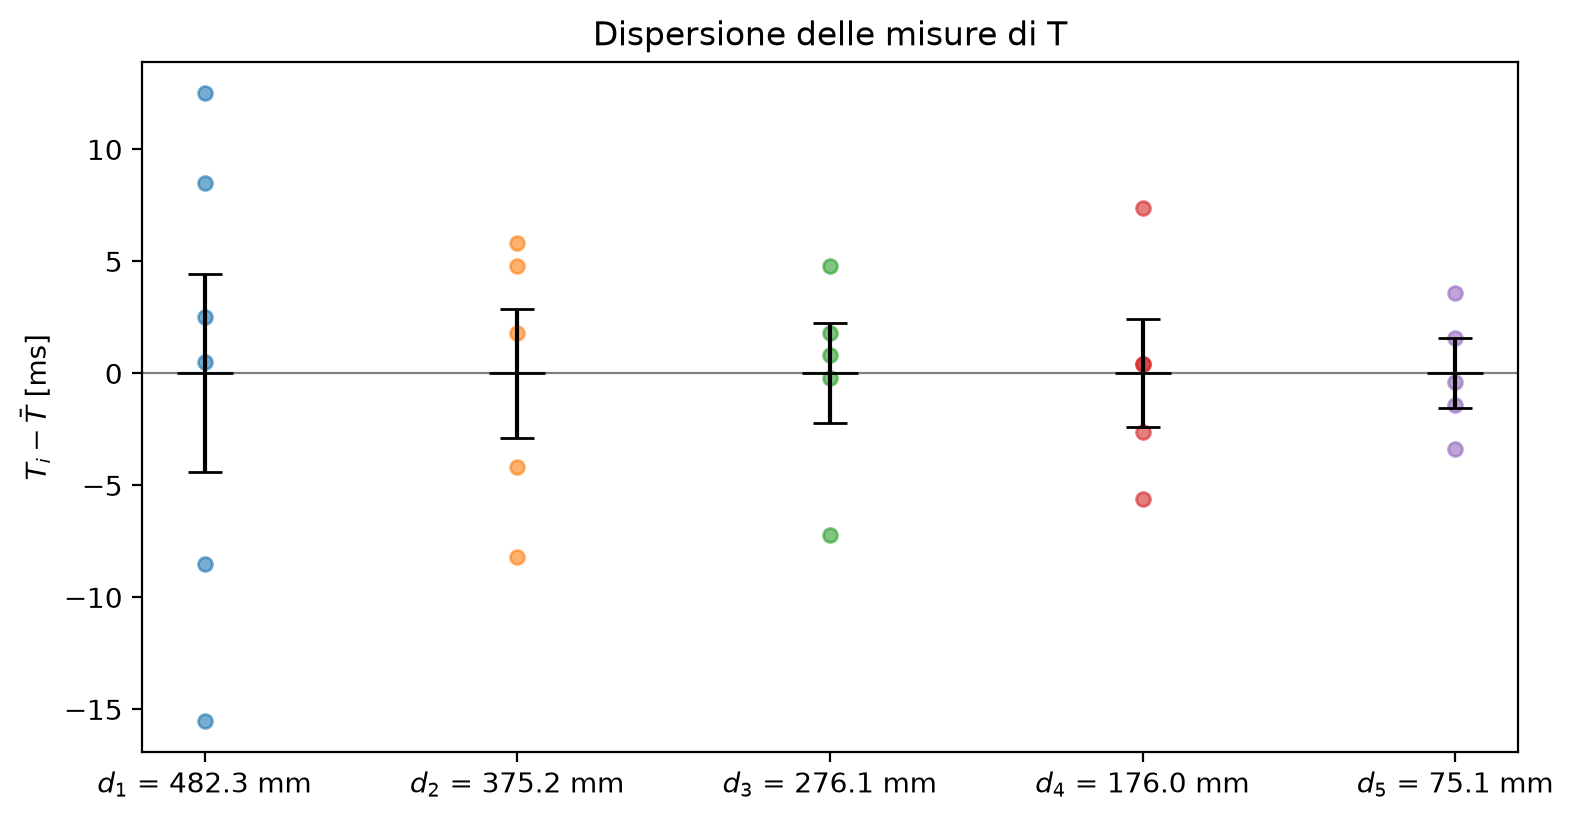
\includegraphics[width=\linewidth]{grafici/disperione_periodo.png}
    \caption{Scarto di ciascuna misura del periodo dalla media del proprio gruppo. Le barre nere indicano l'incertezza $\sigma_T$ sul periodo medio (tabella~\ref{tab:periodi}).}
    \label{fig:dispersione}
\end{figure}

\subsection{Fit del periodo in funzione di $d$}\label{sec:fit}

Abbiamo poi fatto il fit dei valori centrali dei periodi con il modello del pendolo fisico~\eqref{eq:periodo}, lasciando come unico parametro libero la lunghezza dell'asta $l$ e fissando $g = 9.805$~m/s$^2$. Come incertezze sulle ordinate abbiamo usato le $\sigma_T$ della tabella~\ref{tab:periodi}; le incertezze su $d$ non sono incluse nel fit. Il risultato è riportato in figura~\ref{fig:fit_periodo}; i residui, calcolati con la~\eqref{eq:residui}, sono in tabella~\ref{tab:residui} e il confronto tra le lunghezze in tabella~\ref{tab:confronto_l}.

\begin{figure}[!htb]
    \centering
    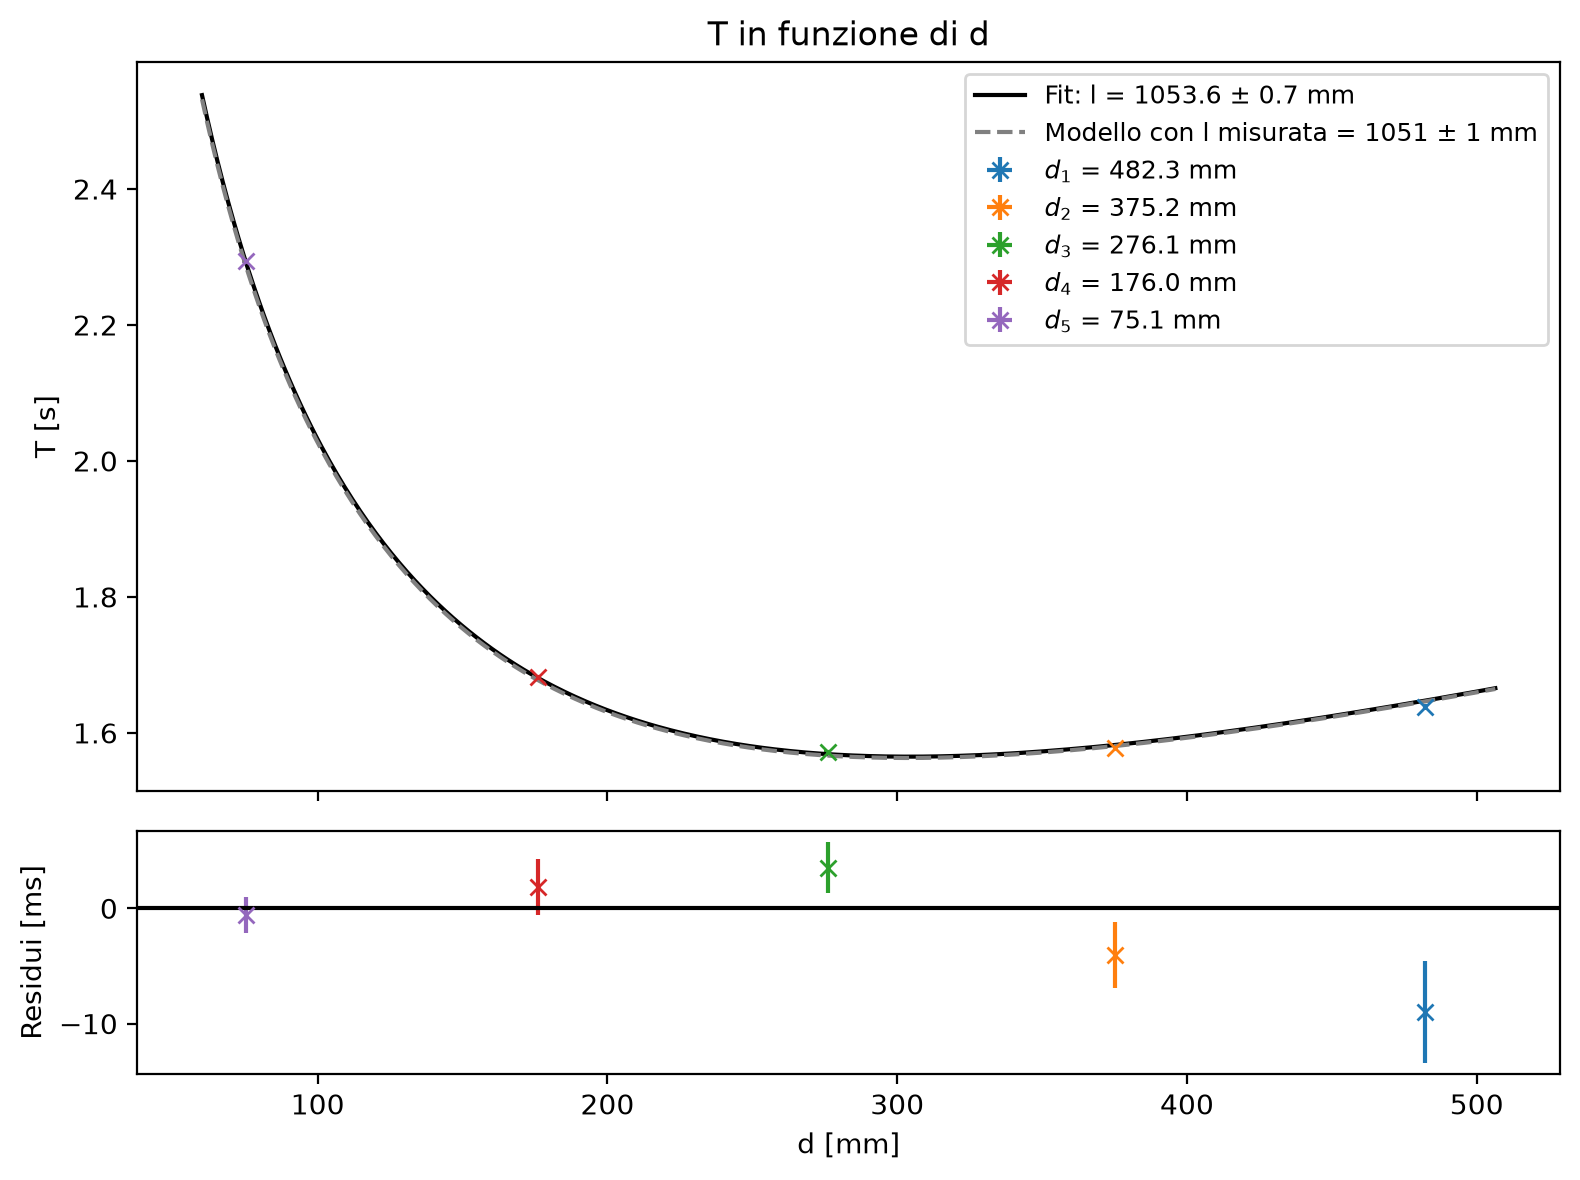
\includegraphics[width=\linewidth]{grafici/fit_periodo.png}
    \caption{In alto: periodo in funzione della distanza $d$, con la curva di best-fit (linea continua) e il modello~\eqref{eq:periodo} calcolato con la lunghezza misurata dell'asta (linea tratteggiata). In basso: residui del fit, con barre d'errore pari a $\sigma_T$.}
    \label{fig:fit_periodo}
\end{figure}

\begin{table}[H]
    \centering
    \begin{tabular}{c|c}
      & residuo (ms)\\
      \hline
      $d_1$ & $-9.0 \pm 4.4$ \\
      $d_2$ & $-4.0 \pm 2.9$ \\
      $d_3$ & $+3.5 \pm 2.2$ \\
      $d_4$ & $+1.8 \pm 2.4$ \\
      $d_5$ & $-0.5 \pm 1.6$ \\
    \end{tabular}
    \caption{Residui del fit~\eqref{eq:residui}, con incertezza pari a $\sigma_T$.}
    \label{tab:residui}
\end{table}

\begin{table}[H]
    \centering
    \begin{tabular}{c|c}
      & $l\pm\sigma_l$ (mm)\\
      \hline
      Best-fit \^{l} & $1053.6 \pm 0.7$ \\
      Misurata con il metro & $1051 \pm 1$ \\
    \end{tabular}
    \caption{Confronto tra la lunghezza dell'asta ottenuta dal fit e quella misurata direttamente (tabella~\ref{tab:asta}).}
    \label{tab:confronto_l}
\end{table}

Dal fit otteniamo $\hat{l} = 1053.6 \pm 0.7$~mm, mentre la lunghezza misurata con il metro è $l = 1051 \pm 1$~mm. La differenza è di 2.6~mm, cioè circa lo 0.25\%, ma siccome entrambe le incertezze sono piccole, applicando la~\eqref{eq:z}, corrisponde a
\begin{equation}
    z = \frac{|\hat{l} - l|}{\sqrt{\sigma_{\hat{l}}^2 + \sigma_l^2}} \simeq 2.2,
    \label{eq:z_fit}
\end{equation}
quindi i due valori non sono pienamente compatibili, anche se non sono nemmeno in netto disaccordo. Come si vede in figura~\ref{fig:fit_periodo}, le due curve sono comunque praticamente sovrapposte sulla scala del grafico e passano molto vicino a tutti i punti. Il minimo previsto dal modello~\eqref{eq:periodo} si trova a $d^* = \hat{l}/\sqrt{12} \simeq 304$~mm, cioè tra $d_3$ e $d_2$, dove infatti abbiamo misurato i periodi più brevi (tabella~\ref{tab:periodi}).

I residui (tabella~\ref{tab:residui}) sono tutti entro circa due volte la loro incertezza dallo zero. Si vede però una leggera tendenza: sono negativi per le due distanze più grandi e positivi o quasi nulli per le altre. Il residuo più grande è quello di $d_1$, che è anche la serie con la dispersione maggiore. Inoltre nel fit non abbiamo considerato le incertezze su $d$, quindi l'incertezza su $\hat{l}$ è probabilmente sottostimata.

\subsection{Correzione per l'ampiezza}\label{sec:ampiezza}
Come abbiamo visto nella sezione~\ref{sec:misure_dirette}, l'ampiezza iniziale di circa 16° è più grande del limite~\eqref{eq:limite_ampiezza} delle piccole oscillazioni. Per la~\eqref{eq:sviluppo_ampiezza}, un'ampiezza maggiore al limite allunga tutti i periodi più o meno dello stesso fattore $1 + \theta_0^2/16$, e quindi fa venire un $\hat{l}$ più grande di quello vero. Per vedere quanto conta abbiamo corretto i periodi misurati con
\begin{equation}
    T_0 = \frac{T}{1 + \theta^2/16}
    \label{eq:correzione_ampiezza}
\end{equation}
(derivata dalla~\eqref{eq:sviluppo_ampiezza}) e rifatto il fit con il modello~\eqref{eq:periodo}. Il problema è che non sappiamo bene quale sia l'ampiezza media durante le 10 oscillazioni, perché diminuisce per l'attrito e noi abbiamo misurato solo quella iniziale. Abbiamo quindi preso $\theta = (12 \pm 4)$°, cioè un intervallo tra 8° e 16°. I risultati sono in tabella~\ref{tab:ampiezza}.

\begin{table}[H]
    \centering
    \begin{tabular}{c|c|c}
      $\theta$ & correzione relativa & $\hat{l}$ (mm)\\
      \hline
      8° & 0.12\% & 1052.1 \\
      12° & 0.27\% & 1050.2 \\
      16° & 0.49\% & 1047.6 \\
    \end{tabular}
    \caption{Lunghezza di best-fit ottenuta correggendo i periodi con la~\eqref{eq:correzione_ampiezza} per diverse ampiezze medie.}
    \label{tab:ampiezza}
\end{table}

Prendendo il valore centrale e come errore sistematico metà della differenza tra il valore più grande e quello più piccolo, otteniamo
\begin{equation}
    \hat{l} = (1050.2 \pm 0.7_{\mathrm{stat}} \pm 2.3_{\mathrm{sist}})\ \text{mm}
    \label{eq:l_corretto}
\end{equation}
che sommando gli errori in quadratura diventa $$\hat{l} = (1050.2 \pm 2.4)~\text{mm}$$. Confrontandolo con la lunghezza misurata (tabella~\ref{tab:confronto_l}) tramite la~\eqref{eq:z} viene $z \simeq 0.3$. La correzione quindi va nella direzione giusta e avvicina il valore del fit a quello misurato, però l'errore sistematico dovuto al fatto che non conosciamo bene l'ampiezza è il più grande di tutti.


\section{Conclusioni}\label{sec:conclusioni}

In questa esperienza abbiamo studiato la dipendenza del periodo di un pendolo fisico dalla distanza $d$ tra il perno e il centro di massa, misurando il periodo per cinque valori di $d$ compresi tra 75 e 482~mm (tabella~\ref{tab:periodi}). L'andamento che abbiamo osservato è in accordo con il modello del pendolo fisico~\eqref{eq:periodo}: il periodo diminuisce al crescere di $d$ fino a un minimo e poi torna a crescere. Il minimo previsto dal modello si trova a $d = l/\sqrt{12}$, cioè a circa 304~mm per la nostra asta, tra $d_3$ e $d_2$, dove infatti abbiamo misurato i periodi più brevi.

Dal fit con $l$ come unico parametro libero abbiamo ottenuto $\hat{l} = 1053.6 \pm 0.7$~mm, mentre la lunghezza misurata con il metro \`e $l = 1051 \pm 1$~mm (tabella~\ref{tab:confronto_l}). La differenza è di circa lo 0.25\%, ma corrisponde a circa $2.2\,\sigma$ (equazione~\eqref{eq:z_fit}), quindi i due valori non sono pienamente compatibili, anche se non sono in netto disaccordo. I residui (tabella~\ref{tab:residui}) sono tutti entro circa due volte la loro incertezza, anche se c'è una leggera tendenza: sono negativi per le due distanze più grandi.

La presenza dei fori nell'asta non sembra essere la causa di questo scarto. Come abbiamo visto nella sezione~\ref{sec:misure_dirette}, i fori rappresentano circa l'1.1\% della massa (equazione~\eqref{eq:epsilon}) e spostano il centro di massa di circa 0.3~mm (equazione~\eqref{eq:spostamento_cm}), meno delle incertezze su $d$. L'effetto più importante è invece l'ampiezza delle oscillazioni. Durante l'esperienza avevamo calcolato male l'ampiezza massima da usare: il limite giusto, dato dalla~\eqref{eq:limite_ampiezza}, è tra 6° e 12°, mentre noi abbiamo fatto partire l'asta da circa 16°. Correggendo i periodi per un'ampiezza media di $(12 \pm 4)$° (sezione~\ref{sec:ampiezza}) otteniamo $\hat{l} = (1050.2 \pm 0.7_{\mathrm{stat}} \pm 2.3_{\mathrm{sist}})$~mm (equazione~\eqref{eq:l_corretto}), compatibile con il valore misurato ($z \simeq 0.3$), ma con un errore sistematico grande perché non abbiamo misurato bene l'ampiezza. Notiamo inoltre che le distanze $d_1$ e $d_2$, che hanno residui negativi, sono state misurate con il calibro, mentre $d_3$, $d_4$ e $d_5$ con il metro: anche un errore sistematico legato al cambio di strumento potrebbe contribuire all'andamento dei residui. Infine, nel fit abbiamo usato solo le incertezze sul periodo e non quelle su $d$, quindi l'incertezza su $\hat{l}$ è probabilmente sottostimata.

In conclusione, il modello del pendolo fisico descrive bene l'andamento del periodo in funzione di $d$, e ci ha permesso di ricavare la lunghezza dell'asta in accordo con la misura diretta.
\end{document}